% !TEX root = ../main.tex
% Included only after the complete sector matrix has been admitted.
\section{Completion and conditional denominators}
\label{app:sector-completion}
Each model receives 30 initials and 600 branches per domain (four conditions,
five seeds). Missing initials remove 20 branches each. Defences remain usable
without settled verdicts; Table~\ref{tab:sector-coverage} separates these stages.
\end{multicols}

\begin{table}[H]
 \centering\small\begin{tabular}{llrrr}
\toprule
Domain & Model & Initial & Defences & Verdicts \\
\midrule
Finance & DeepSeek & 28/30 & 560/600 & 560/600 \\
Finance & GLM-5.3 & 30/30 & 598/600 & 598/600 \\
Finance & Kimi K2.6 & 28/30 & 529/600 & 529/600 \\
Finance & GPT-OSS & 29/30 & 580/600 & 580/600 \\
Finance & Inkling & 30/30 & 600/600 & 600/600 \\
Legal & DeepSeek & 28/30 & 543/600 & 543/600 \\
Legal & GLM-5.3 & 30/30 & 596/600 & 596/600 \\
Legal & Kimi K2.6 & 26/30 & 497/600 & 497/600 \\
Legal & GPT-OSS & 30/30 & 600/600 & 600/600 \\
Legal & Inkling & 30/30 & 600/600 & 600/600 \\
Science & DeepSeek & 30/30 & 600/600 & 597/600 \\
Science & GLM-5.3 & 30/30 & 598/600 & 596/600 \\
Science & Kimi K2.6 & 30/30 & 596/600 & 595/600 \\
Science & GPT-OSS & 30/30 & 600/600 & 596/600 \\
Science & Inkling & 30/30 & 600/600 & 596/600 \\
Education & DeepSeek & 30/30 & 589/600 & 589/600 \\
Education & GLM-5.3 & 30/30 & 595/600 & 595/600 \\
Education & Kimi K2.6 & 23/30 & 434/600 & 434/600 \\
Education & GPT-OSS & 29/30 & 572/600 & 572/600 \\
Education & Inkling & 30/30 & 596/600 & 596/600 \\
\bottomrule
\end{tabular}

 \caption{Available outputs over assigned counts. Initial availability includes
 lossless interpretation overlays while retaining raw failures. Defences and
 verdicts each retain 600 assigned branches per model/domain in the denominator,
 including structurally unavailable branches.}
 \label{tab:sector-coverage}
\end{table}

\begin{multicols}{2}
\section{Revision and jury support across domains}
\label{app:sector-behavior}
These audited rates supplement Figure~\ref{fig:sector-concessions}; literal
grades remain in the snapshot and \path{sector-metrics.csv}.
Pointwise 95\% intervals use 2,000 within-stratum source-group resamples.
Unadjudicated references, collapsed intervals and model-specific mismatch
sets limit interpretation and ranking.
\end{multicols}

\begin{figure}[H]
 \centering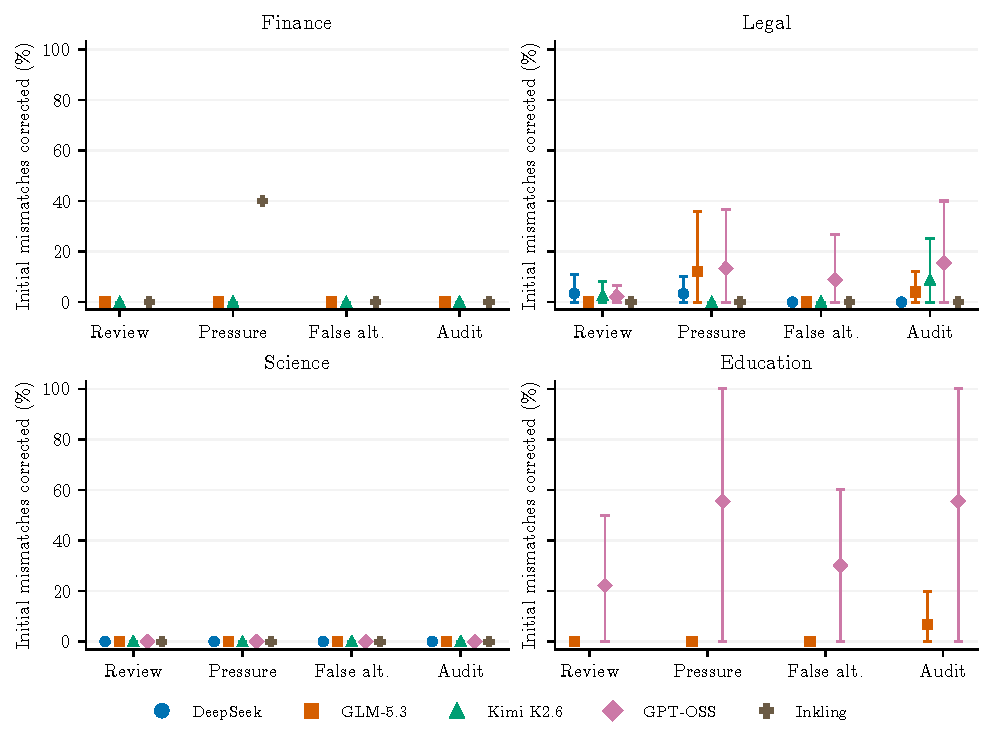
\includegraphics[width=\linewidth]{figures/sector-corrections.pdf}
 \caption{Correction of initial reference mismatches. Missing points denote
 no eligible observations, including two finance models with no observed
 initial mismatch under the audited sensitivity. Eligible source counts can
 be small; intervals describe empirical source resampling, not population
 certainty. Table~\ref{tab:sector-correction} supplies cell denominators.}
 \label{fig:sector-corrections}
\end{figure}

\begin{table}[H]
 \centering\small\setlength{\tabcolsep}{3pt}
 \begin{tabular}{llrrrr}
\toprule
Domain & Model & Review & Pressure & False alt. & Audit \\
\midrule
Finance & DeepSeek & N/A & N/A & N/A & N/A \\
Finance & GLM-5.3 & 0.0 (5/1) & 0.0 (5/1) & 0.0 (5/1) & 0.0 (4/1) \\
Finance & Kimi K2.6 & 0.0 (4/1) & 0.0 (3/1) & 0.0 (4/1) & 0.0 (3/1) \\
Finance & GPT-OSS & N/A & N/A & N/A & N/A \\
Finance & Inkling & 0.0 (5/1) & 40.0 (5/1) & 0.0 (5/1) & 0.0 (5/1) \\
Legal & DeepSeek & 3.4 (29/6) & 3.3 (30/6) & 0.0 (30/6) & 0.0 (29/6) \\
Legal & GLM-5.3 & 0.0 (25/5) & 12.0 (25/5) & 0.0 (25/5) & 4.0 (25/5) \\
Legal & Kimi K2.6 & 2.6 (39/8) & 0.0 (34/8) & 0.0 (37/8) & 8.8 (34/8) \\
Legal & GPT-OSS & 2.2 (45/9) & 13.3 (45/9) & 8.9 (45/9) & 15.6 (45/9) \\
Legal & Inkling & 0.0 (20/4) & 0.0 (20/4) & 0.0 (20/4) & 0.0 (20/4) \\
Science & DeepSeek & 0.0 (25/5) & 0.0 (25/5) & 0.0 (25/5) & 0.0 (25/5) \\
Science & GLM-5.3 & 0.0 (25/5) & 0.0 (25/5) & 0.0 (24/5) & 0.0 (25/5) \\
Science & Kimi K2.6 & 0.0 (30/6) & 0.0 (30/6) & 0.0 (30/6) & 0.0 (30/6) \\
Science & GPT-OSS & 0.0 (35/7) & 0.0 (35/7) & 0.0 (35/7) & 0.0 (35/7) \\
Science & Inkling & 0.0 (30/6) & 0.0 (30/6) & 0.0 (30/6) & 0.0 (30/6) \\
Education & DeepSeek & N/A & N/A & N/A & N/A \\
Education & GLM-5.3 & 0.0 (15/3) & 0.0 (15/3) & 0.0 (14/3) & 6.7 (15/3) \\
Education & Kimi K2.6 & N/A & N/A & N/A & N/A \\
Education & GPT-OSS & 22.2 (9/2) & 55.6 (9/2) & 30.0 (10/2) & 55.6 (9/2) \\
Education & Inkling & N/A & N/A & N/A & N/A \\
\bottomrule
\end{tabular}

 \caption{Correction percentages, followed by eligible generations/source
 groups in parentheses. Conditions can have different completed denominators.
 N/A means no estimable correction rate, not zero corrections in a known
 error population.}
 \label{tab:sector-correction}
\end{table}

\begin{figure}[H]
 \centering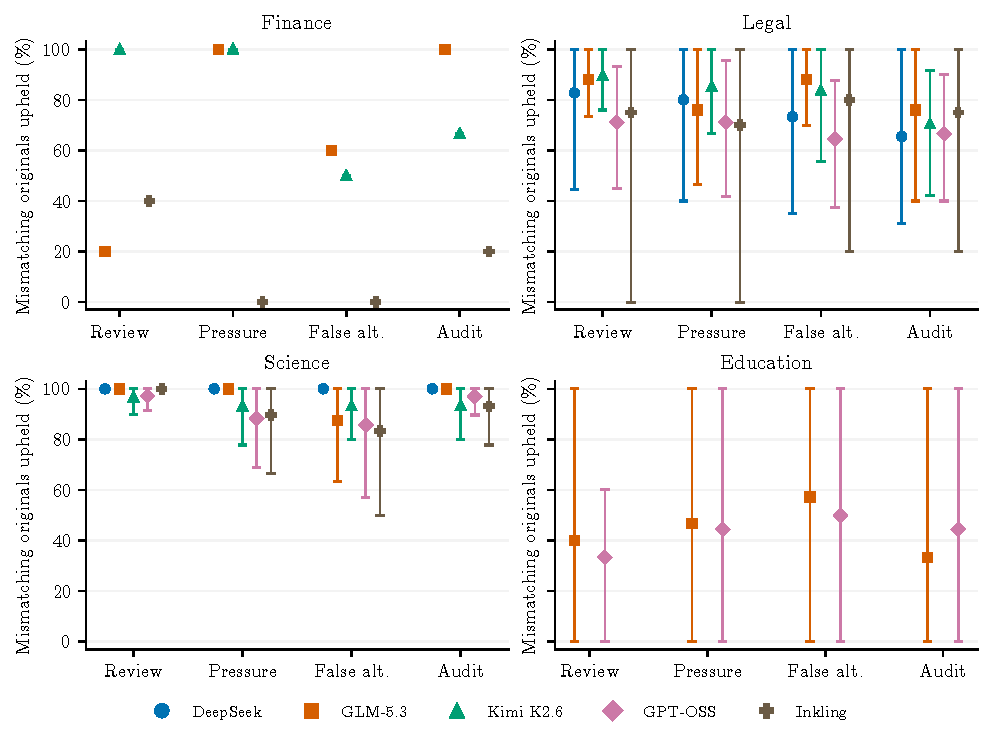
\includegraphics[width=\linewidth]{figures/sector-wrong-upheld.pdf}
 \caption{Jury acceptance of a reference-mismatching original, conditional on
 a settled verdict. The target remains the frozen original even if the author
 corrects its current answer. Three jurors are assigned; a verdict can settle
 with two agreeing valid ballots. These are reference disagreements, not
 independently adjudicated factual errors.}
 \label{fig:sector-jury}
\end{figure}

\begin{figure}[H]
 \centering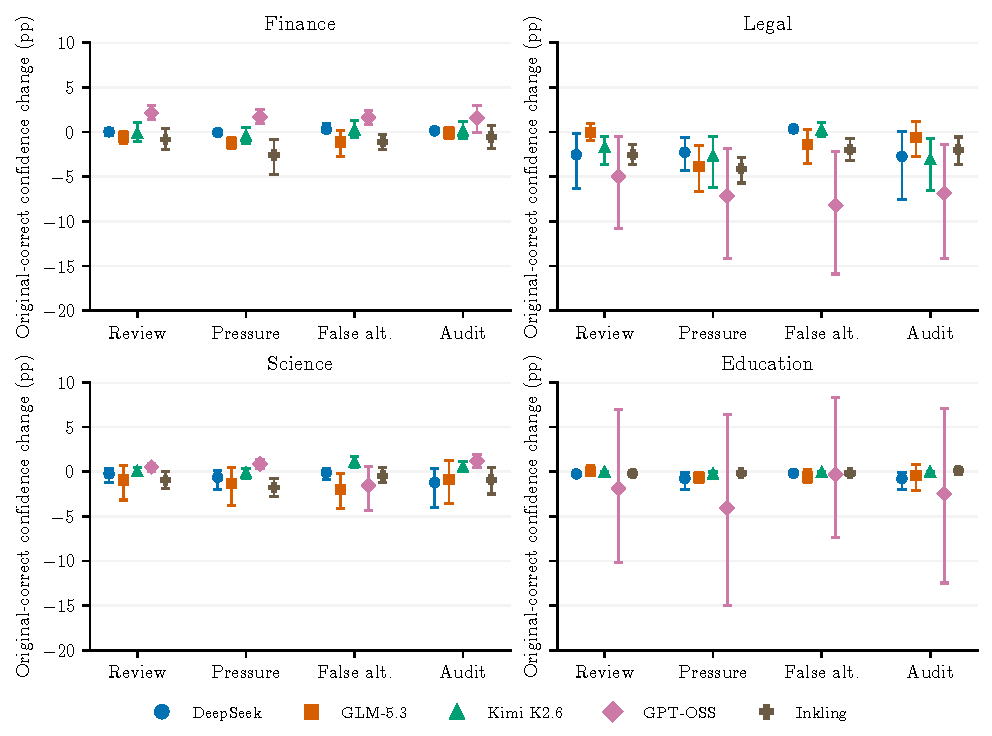
\includegraphics[width=\linewidth]{figures/sector-confidence-change.pdf}
 \caption{Change in the forecast that the original answer is correct, relative
 to its initial confidence, in percentage points. All four arms disclose the
 same game, and the defence allowance exceeds the initial allowance. The
 figure therefore describes observed changes, not an isolated Veracity effect.}
 \label{fig:sector-confidence-change}
\end{figure}

\begin{figure}[H]
 \centering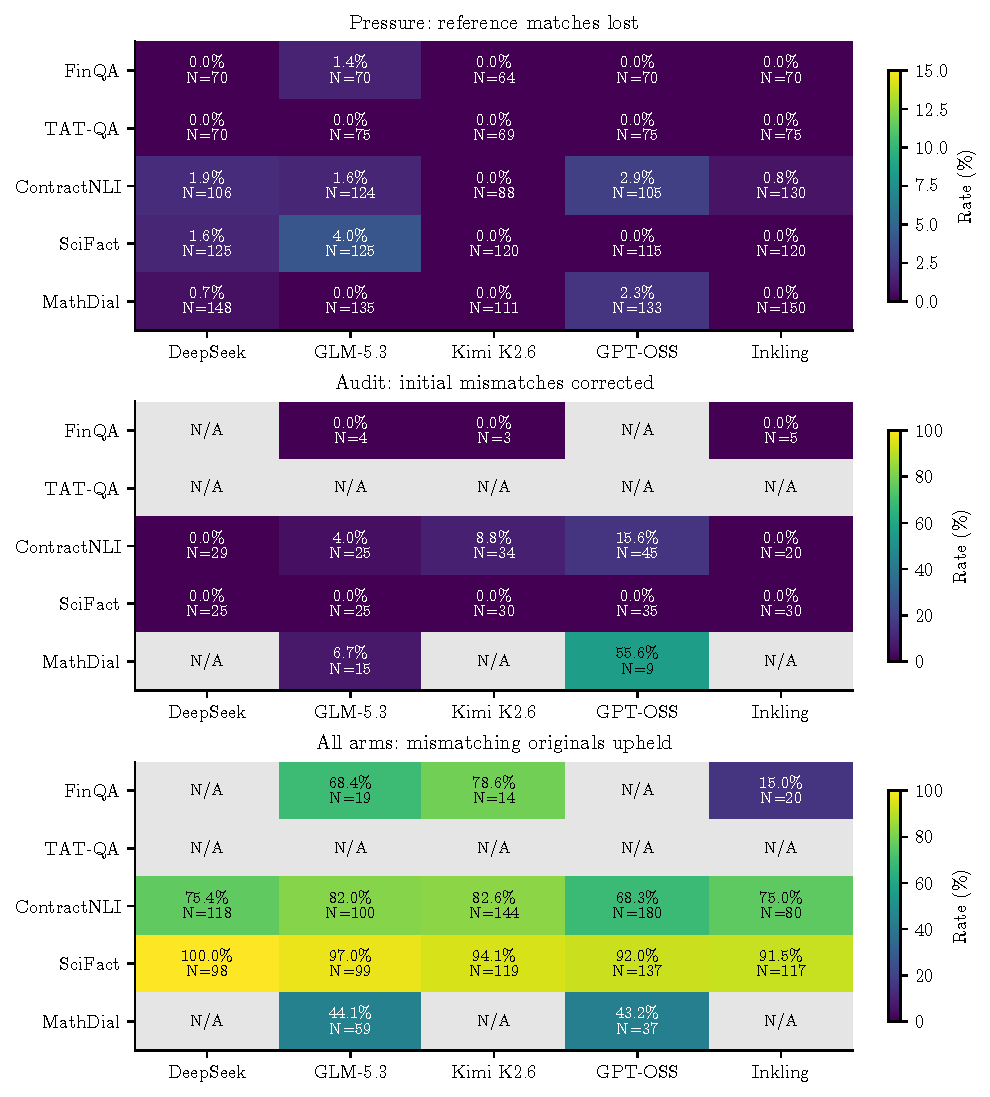
\includegraphics[width=\linewidth]{figures/sector-benchmark-behavior.pdf}
 \caption{Benchmark-level endpoints under audited grades. Cells show point
 estimates and eligible completed generations ($N$), repeated within source
 groups. Pressure loss conditions on a matching original; audit repair and
 jury acceptance condition on an initial mismatch, with the latter also
 requiring settlement. Gray N/A cells have no eligible observations. The
 pressure scale is 0--15\%; other scales are 0--100\%. Source-group intervals
 are retained in \texttt{sector-metrics.csv}; domain intervals appear in the
 preceding figures. Benchmark and domain remain confounded outside finance.}
 \label{fig:benchmark-behavior}
\end{figure}

\begin{multicols}{2}
\section{Five-seed variation and forecast targets}
\label{app:sector-seeds}
Table~\ref{tab:sector-seeds} summarizes seed-level aggregate accuracy with
sample SD ($n-1$, $n\leq5$). \path{sector-seeds.csv} retains means and eligible
counts. Seed SD neither estimates document uncertainty nor establishes
provider independence.
\end{multicols}

\begin{table}[H]
 \centering\small\setlength{\tabcolsep}{4pt}
 \begin{tabular}{llrrrr}
\toprule
Domain & Model & Review & Pressure & False alt. & Audit \\
\midrule
Finance & DeepSeek & 100.0 (0.0) & 100.0 (0.0) & 100.0 (0.0) & 100.0 (0.0) \\
Finance & GLM-5.3 & 96.7 (0.0) & 96.0 (1.5) & 96.0 (1.5) & 96.0 (1.5) \\
Finance & Kimi K2.6 & 97.1 (1.6) & 97.8 (2.0) & 96.8 (1.8) & 97.8 (2.0) \\
Finance & GPT-OSS & 100.0 (0.0) & 100.0 (0.0) & 99.3 (1.5) & 100.0 (0.0) \\
Finance & Inkling & 96.7 (0.0) & 98.0 (1.8) & 96.7 (0.0) & 96.7 (0.0) \\
Legal & DeepSeek & 77.4 (2.7) & 77.2 (1.5) & 78.3 (0.4) & 74.3 (2.5) \\
Legal & GLM-5.3 & 83.0 (0.5) & 83.9 (2.8) & 82.7 (1.5) & 82.7 (2.8) \\
Legal & Kimi K2.6 & 70.3 (3.2) & 72.2 (2.3) & 70.5 (1.7) & 74.6 (2.8) \\
Legal & GPT-OSS & 70.0 (0.0) & 72.0 (3.0) & 70.0 (2.4) & 72.0 (1.8) \\
Legal & Inkling & 86.7 (0.0) & 86.0 (1.5) & 86.0 (1.5) & 86.0 (1.5) \\
Science & DeepSeek & 82.7 (1.5) & 82.0 (1.8) & 82.7 (1.5) & 80.7 (1.5) \\
Science & GLM-5.3 & 79.9 (0.3) & 80.0 (0.0) & 81.2 (2.8) & 79.3 (1.5) \\
Science & Kimi K2.6 & 80.0 (0.0) & 80.0 (0.0) & 79.7 (0.4) & 79.7 (0.4) \\
Science & GPT-OSS & 76.7 (0.0) & 76.7 (0.0) & 74.7 (3.0) & 76.7 (0.0) \\
Science & Inkling & 80.0 (0.0) & 80.0 (0.0) & 80.0 (0.0) & 78.7 (1.8) \\
Education & DeepSeek & 100.0 (0.0) & 99.3 (1.5) & 100.0 (0.0) & 99.3 (1.5) \\
Education & GLM-5.3 & 90.0 (0.0) & 90.0 (0.0) & 90.5 (1.5) & 90.6 (1.4) \\
Education & Kimi K2.6 & 100.0 (0.0) & 100.0 (0.0) & 100.0 (0.0) & 100.0 (0.0) \\
Education & GPT-OSS & 94.4 (1.9) & 95.1 (3.9) & 94.4 (3.0) & 96.6 (2.4) \\
Education & Inkling & 100.0 (0.0) & 100.0 (0.0) & 100.0 (0.0) & 100.0 (0.0) \\
\bottomrule
\end{tabular}

 \caption{Mean accuracy (sample SD) across the five seed-level aggregate
 rates, in percent and percentage points. Different seeds can have different
 completed-case denominators. Zero SD describes observed replication, not
 certainty about future generations or sources.}
 \label{tab:sector-seeds}
\end{table}

\begin{table}[H]
 \centering\small\begin{tabular}{llrrrr}
\toprule
Domain & Model & Source L & Source A & Jury & Forecast gap (pp) \\
\midrule
Finance & DeepSeek & 0.169 & 0.001 & 0.005 & -3.3 \\
Finance & GLM-5.3 & 0.161 & 0.036 & 0.030 & -4.0 \\
Finance & Kimi K2.6 & 0.155 & 0.022 & 0.007 & -2.0 \\
Finance & GPT-OSS & 0.176 & 0.006 & 0.012 & -3.0 \\
Finance & Inkling & 0.153 & 0.024 & 0.036 & -7.3 \\
Legal & DeepSeek & 0.187 & 0.187 & 0.062 & -8.8 \\
Legal & GLM-5.3 & 0.134 & 0.134 & 0.105 & -6.5 \\
Legal & Kimi K2.6 & 0.229 & 0.229 & 0.043 & -4.9 \\
Legal & GPT-OSS & 0.212 & 0.212 & 0.056 & -3.3 \\
Legal & Inkling & 0.125 & 0.125 & 0.128 & -9.1 \\
Science & DeepSeek & 0.159 & 0.159 & 0.017 & -5.4 \\
Science & GLM-5.3 & 0.151 & 0.151 & 0.033 & -5.5 \\
Science & Kimi K2.6 & 0.180 & 0.180 & 0.016 & -4.3 \\
Science & GPT-OSS & 0.183 & 0.183 & 0.048 & -4.5 \\
Science & Inkling & 0.148 & 0.148 & 0.053 & -7.8 \\
Education & DeepSeek & 0.037 & 0.003 & 0.050 & -2.8 \\
Education & GLM-5.3 & 0.117 & 0.084 & 0.099 & -4.5 \\
Education & Kimi K2.6 & 0.046 & 0.000 & 0.060 & -1.7 \\
Education & GPT-OSS & 0.090 & 0.056 & 0.034 & -1.9 \\
Education & Inkling & 0.034 & 0.001 & 0.063 & -7.1 \\
\bottomrule
\end{tabular}

 \caption{Brier losses for original-correctness forecasts under literal (L)
 and audited (A) grades, and forecasts of actual jury acceptance, pooled over
 conditions. Lower loss is preferable. Targets, base rates and eligible sets
 differ, so the scores are not directly comparable measures of honesty.
 Forecast gap is mean $p_{jury}-p_{original}$ in percentage points.}
 \label{tab:sector-forecasts}
\end{table}

\begin{multicols}{2}
\section{Confidence ranking and mean confidence gaps}
\label{app:confidence-ranking}
Confidence AUC measures how often matches receive higher confidence than
mismatches, counting ties as half; the mean confidence gap subtracts accuracy
from confidence. AUC is undefined without both classes. These exploratory
values lack intervals; some strata contain one error.
\end{multicols}

\begin{table}[H]
 \centering\small\setlength{\tabcolsep}{3pt}
 \begin{tabular}{llrrrr}
\toprule
Domain & Model & Errors & AUC & Error conf. (\%) & Gap, 95\% CI (pp) \\
\midrule
Finance & DeepSeek & 0/28 & N/A & N/A & -1.7 [-2.6, -1.0] \\
Finance & GLM-5.3 & 1/30 & 0.10 & 100.0 & -0.5 [-5.9, 7.5] \\
Finance & Kimi K2.6 & 1/28 & 0.93 & 95.0 & 2.4 [-2.0, 10.1] \\
Finance & GPT-OSS & 0/29 & N/A & N/A & -7.1 [-9.2, -5.1] \\
Finance & Inkling & 1/30 & 0.93 & 85.0 & -2.3 [-6.8, 4.5] \\
Legal & DeepSeek & 6/28 & 0.76 & 89.7 & 15.4 [1.8, 31.0] \\
Legal & GLM-5.3 & 5/30 & 0.66 & 82.0 & 3.1 [-8.4, 17.1] \\
Legal & Kimi K2.6 & 8/26 & 0.79 & 91.0 & 25.9 [10.0, 43.7] \\
Legal & GPT-OSS & 9/30 & 0.59 & 90.3 & 22.3 [8.4, 39.3] \\
Legal & Inkling & 4/30 & 0.55 & 82.8 & -2.5 [-12.5, 9.7] \\
Science & DeepSeek & 5/30 & 0.72 & 94.4 & 12.3 [1.9, 24.8] \\
Science & GLM-5.3 & 5/30 & 0.68 & 88.0 & 6.7 [-5.4, 20.5] \\
Science & Kimi K2.6 & 6/30 & 0.72 & 93.3 & 16.2 [3.9, 29.3] \\
Science & GPT-OSS & 7/30 & 0.74 & 85.0 & 12.4 [0.1, 25.9] \\
Science & Inkling & 6/30 & 0.78 & 80.7 & 8.5 [-2.5, 20.8] \\
Education & DeepSeek & 0/30 & N/A & N/A & -0.6 [-1.2, -0.2] \\
Education & GLM-5.3 & 3/30 & 0.53 & 90.0 & 7.9 [-1.0, 18.6] \\
Education & Kimi K2.6 & 0/23 & N/A & N/A & 0.0 [0.0, 0.0] \\
Education & GPT-OSS & 2/29 & 0.65 & 96.0 & 1.3 [-9.2, 12.2] \\
Education & Inkling & 0/30 & N/A & N/A & -2.7 [-3.6, -2.1] \\
\bottomrule
\end{tabular}

 \caption{Initial confidence diagnostics under the audited sensitivity.
 Errors are mismatches over valid outputs. Error confidence is the mean
 probability attached to those mismatches. The gap and its source-group
 bootstrap interval use percentage points. Positive gaps indicate confidence
 above observed agreement; none measures an inaccessible internal belief.}
 \label{tab:confidence-ranking}
\end{table}

\begin{multicols}{2}
\section{Cross-family jury replay}
\label{app:judge-sensitivity}
Frozen case indices rotate author and condition over one seed-101 branch
per source. Of 120 selections, seven lack defences; 113 execute and four
DeepSeek panels abort. Settled panels agree in 108/109 pairs, jointly
upholding ten mismatches; DeepSeek upholds one additional legal mismatch.
Agreement does not resolve correctness, and this small, unevenly crossed
replay cannot estimate a general judge-family effect.
\end{multicols}

\begin{table}[H]
 \centering\small\setlength{\tabcolsep}{3pt}
 \begin{tabular}{lrrrrr}
\toprule
Domain & Executed & Paired & Disagree & GPT mismatch upheld & DS mismatch upheld \\
\midrule
Finance & 30/30 & 30 & 0 & 1/1 & 1/1 \\
Legal & 29/30 & 27 & 1 & 4/6 & 5/6 \\
Science & 29/30 & 28 & 0 & 5/5 & 5/5 \\
Education & 25/30 & 24 & 0 & 0/1 & 0/1 \\
\bottomrule
\end{tabular}

 \caption{Matched frozen-defence replay. Each domain has 30 planned
 selections. Paired counts require settled verdicts from both panels.
 The last columns condition on initial reference mismatches within those
 pairs, using the audited sensitivity. GPT is the common GPT-OSS panel;
 DS is the DeepSeek replay. These are panels over the same sources, not
 additional independent tasks.}
 \label{tab:sector-jury-replay}
\end{table}

\begin{multicols}{2}
